%!TEX root = ../thesis.tex
\documentclass[../thesis]{subfiles}

\begin{document}
	\section{Results}
	\label{sec:multicore:results}

	\tdg{Sugar and methodology}
	Performance measurements are required to verify and quantify the improvements from using the block method over the point one and to properly compare the algorithms for the two presented strategies. This section presents the results obtained for these algorithms with tests running in a single node of the 701 group in the \search\footnote{\url{http://search.di.uminho.pt}} cluster. In addition to what was described in \cref{sec:case:method}, the methodology for these tests also included power-of-two equivalent dimensions (2048, 4096 and 8192). A block dimension of 64 was experimentally found to be the most efficient.

	\tdg{OS and hardware}
	Nodes in this group run Linux CentOS 6.2 with two 8-core \intel\xeon E5-2650 processors and 64GB of shared DRAM (\numa). Each of its processors runs at a clock frequency of 2.00 GHz and has hardware support for 16 simultaneous threads with \intel Hyper-Threading. Further information regarding the hardware in these nodes is shown in \cref{tab:search:701}.

	\tdg{compiler and libraries}
	Tests were built using \intel Composer XE 2011 (compiled with \icpc 12.0.2 and linked with \intel\mkl, for optimized \blas and \lapack) and Armadillo C++ Linear Algebra library (version 3.800.2).

	\begin{table}[!htp]
		\begin{center}
			\begin{tabular}{lr}
				\hline
				Clock frequency & 2.00 GHz \\
				Cores & 8 \\
				SIMD width & 256-bit (\acs{AVX}) \\
				Memory size & 64 GB \\
				\hline
				Peak DP FLOPs & 128 GigaFLOP/s \\
				Peak Memory Bandwidth & 51.2 GB/s \\ 
				\hline
			\end{tabular}
		\end{center}
		\caption[Hardware details for \search group 701 nodes]{Hardware details for \search group 701 nodes (further information available in \cite{Intel:Xeon:e5_2650,Intel:Xeon:e5_2600})}
		\label{tab:search:701}
	\end{table}



	Preliminary tests showed identical results for the column and the row strategy. Consequently, results will are shown only for one of these strategies. As expected, they do not scale at all, unlike the diagonal strategy that reaches its maximum performance when using all the hardware supported threads (\cref{fig:multicore:point:row:times,fig:multicore:point:diagonal:speedup}).

	The block method also scales well (\cref{fig:multicore:block:diagonal:times}), with the maximum speedup versus the point-row implementation being reached when using 32 threads (the 16 cores with Hyper-Threading). Using power-of-two matrices it is possible to see that not only is the block method faster than the point alternative, it is also less sensitive to small variations in the matrix size (\cref{fig:multicore:sensitivity}).


	Blocking already shows significant speedup on its own, when compared to the point method using the same number of threads (\cref{fig:multicore:blocking:speedup}). Nonetheless, \cref{fig:multicore:block:diagonal:speedup:accumulated} shows the scalability of the block method compared with single-threaded point-diagonal achieves impressive speedup values (over 128 using 16 or 32 threads). These values are even higher for particular matrix sizes (\cref{fig:multicore:block:diagonal:speedup:accumulated:strange}).

	\begin{figure}[p]
		\begin{minipage}[t]{0.48\textwidth}
			\centering
			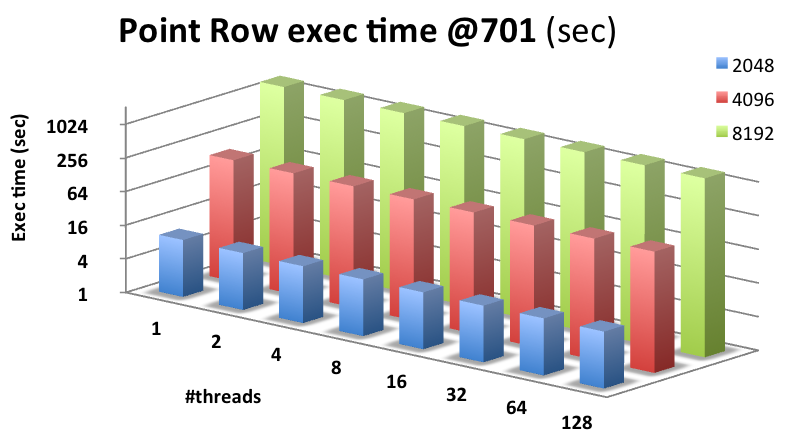
\includegraphics[width=\textwidth]{assets/images/multicore/point-row.png}
			\captionsetup{font=small}
			\caption{Execution times for point-row}
			\label{fig:multicore:point:row:times}
		\end{minipage}
		\hfill
		\begin{minipage}[t]{0.46\textwidth}
			\centering
			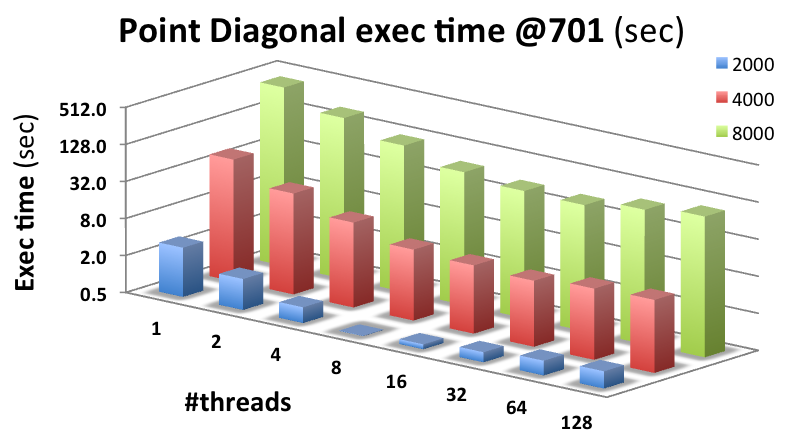
\includegraphics[width=\textwidth]{assets/images/multicore/point-diagonal.png}
			\captionsetup{font=small}
			\caption{Execution times for point-diagonal}
			\label{fig:multicore:point:diagonal:speedup}
		\end{minipage}
	\end{figure}

	\begin{figure}[p]
		\begin{minipage}[t]{0.47\textwidth}
			\centering
			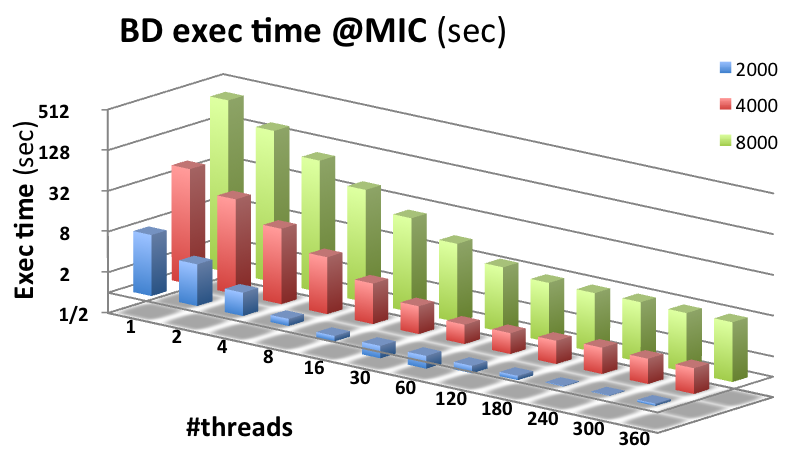
\includegraphics[width=\textwidth]{assets/images/multicore/block-diagonal.png}
			\caption{Execution times for block-diagonal}
			\label{fig:multicore:block:diagonal:times}
		\end{minipage}
		\hfill
		\begin{minipage}[t]{0.48\textwidth}
			\centering
			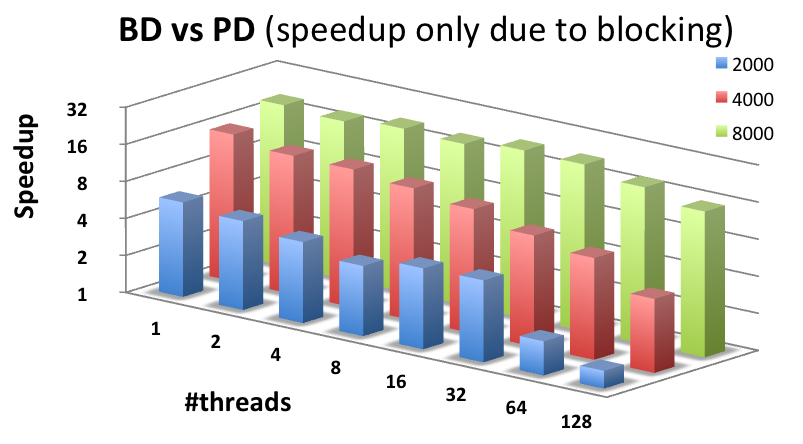
\includegraphics[width=\textwidth]{assets/images/multicore/blocking-speedup.png}
			\caption{Speedups achieved with blocking for diagonal strategy}
			\label{fig:multicore:blocking:speedup}
		\end{minipage}
	\end{figure}

	\begin{figure}[p]
		\centering
		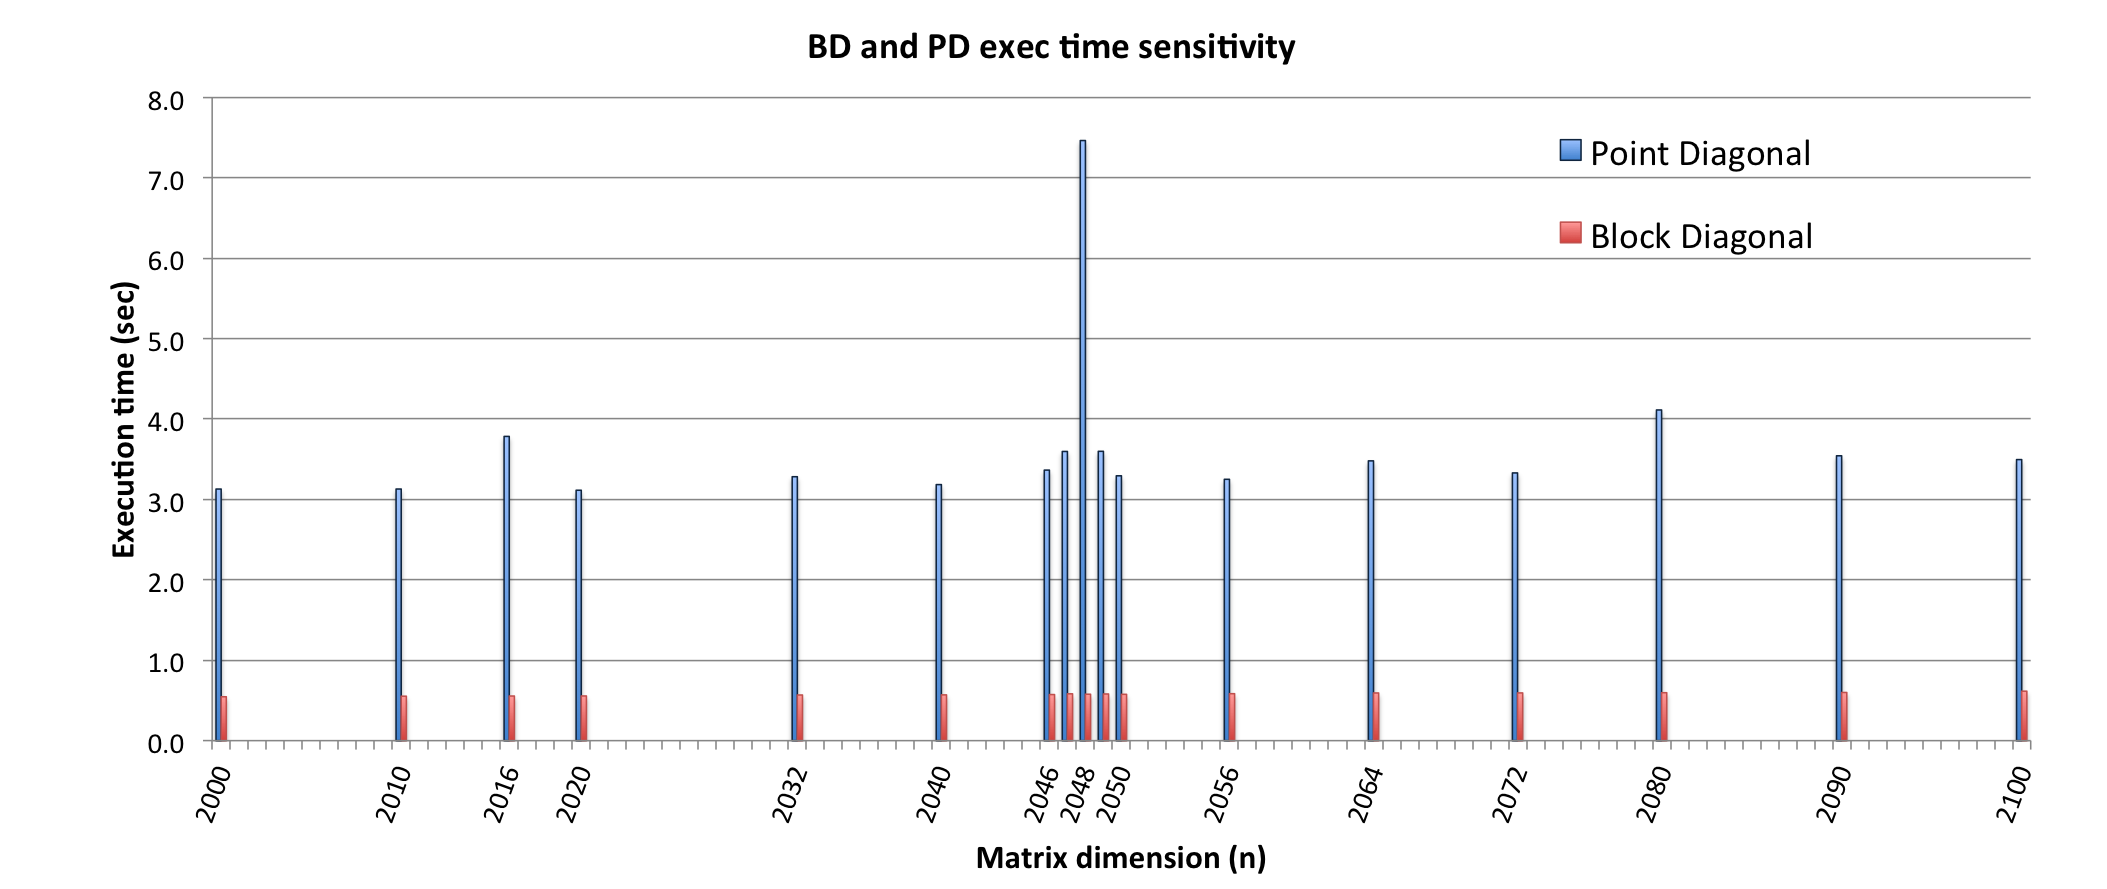
\includegraphics[height=0.28\textheight]{assets/images/multicore/resonance.png}
		\captionsetup{font=small}
		\caption{Execution time sensitivity for both point-diagonal and block-diagonal}
		\label{fig:multicore:sensitivity}
	\end{figure}

	\begin{figure}[!t]
		\begin{minipage}{0.48\textwidth}
			\centering
			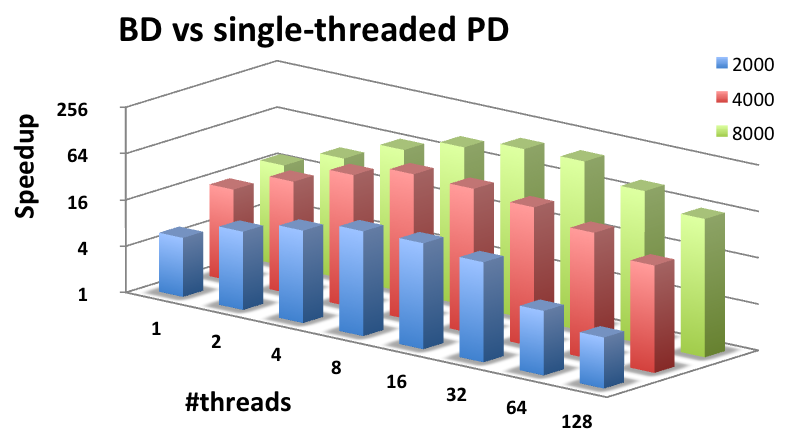
\includegraphics[width=\textwidth]{assets/images/multicore/blocking-multithread-speedup.png}
			\captionsetup{font=small}
			\caption{Accumulated speedup (blocking and parallelism) achieved with diagonal strategy}
			\label{fig:multicore:block:diagonal:speedup:accumulated}
		\end{minipage}
		\hfill
		\begin{minipage}{0.48\textwidth}
			\centering
			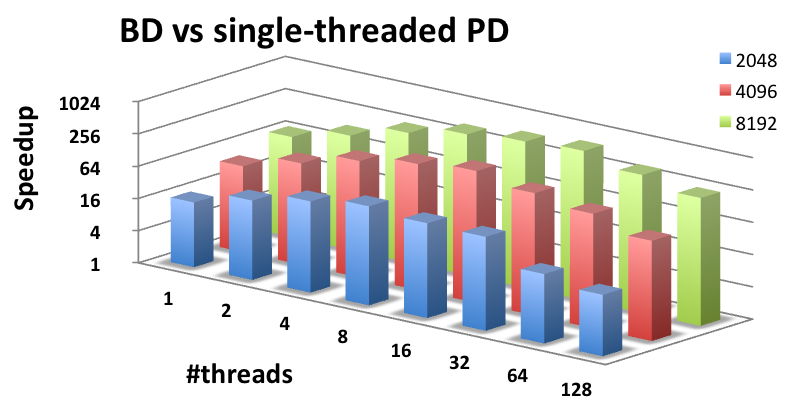
\includegraphics[width=\textwidth]{assets/images/multicore/blocking-multithread-speedup-power2.png}
			\captionsetup{font=small}
			\caption{Accumulated speedup (blocking and parallelism) achieved with diagonal strategy (power of 2 sizes)}
			\label{fig:multicore:block:diagonal:speedup:accumulated:strange}
		\end{minipage}
	\end{figure}
\end{document}
